\documentclass[11]{article}

\usepackage[a4paper,left=3cm,right=2cm,top=2.5cm,bottom=2.5cm]{geometry}
\usepackage{lipsum}
\usepackage{amsmath}
\usepackage{multirow}	
\usepackage{graphicx}


\title{Machine Learning HW5}
\author{Payam AZAD - 503111554}
\begin{document}
\pagenumbering{gobble}
 \maketitle
 
 \begin{table}[ht!]
\centering
\label{my-label}
\begin{tabular}{|ll|l|l|l|l|l|}
\hline
                                             &          & Q1 & Q2 & Q3 & Q4 & Total \\ \hline
\multicolumn{1}{|l|}{\multirow{2}{*}{Grade}} & Max      & 1  & 1 & 2 & 1 &  5     \\ \cline{2-6} 
\multicolumn{1}{|l|}{}                       & Expected & 1  & 2 & 1 & 1 &  5   \\ \hline
\end{tabular}
\end{table}


\section*{Q1}
To run codes Jupyter Notebook is needed. just it have to be loaded into jupyter notebook and each section can be run pressing Shift+Enter and all the resutls are self explanatory.

\section*{Q2}
%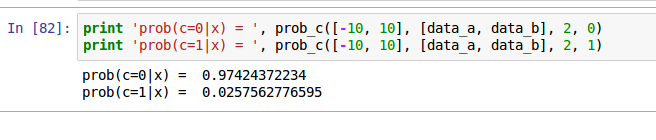
\includegraphics[scale=0.75]{1-b.png} \\
 
\section*{Q3}



\section*{Q4}


 
\end{document}